%! Suppress = InclusionLoop
%% -----------------------------------------------------------------------------

\chapter{Introduction}\label{ch:introduction}

In today's modern society, ...


%% -----------------------------------------------------------------------------

\section{Motivation}\label{sec:motivation}

Modern programming languages like Rust and Go have mechanisms to protect potential
unsafe usages, e.g., dereferences of raw pointers or modifying static variables. Thus, it is
recommended to avoid unsafe usages. However, if a developer wants to avoid unsafe
usages and potential security vulnerabilities caused by these usages, they do not only need
to check their code but also their dependencies.

To provide a developer the power to understand the unsafe usages within their code base,
tools like cargo-geiger~\cite{cargogeiger} exists. Unfortunately, such a tool does not exist by today for Go.
Thus, an in-depth analysis of how many Go projects include direct and indirect unsafe
usages and if these projects are vulnerable does not exist, e.g., to buffer overflows~\cite{larochelle2001, alnaeli2017, wang2020}.
Within this work, the aim is to develop a tool, probably based on go vet~\cite{govet}, that can identify
unsafe usages in Go projects - similar to cargo-geiger. Based on this tool, the thesis should
evaluate how common unsafe usages in Go are and try to analyze if vulnerabilities caused
by unsafe usages exist.


%% -----------------------------------------------------------------------------

\section{Contributions}\label{sec:contributions}

The contributions of this thesis are:

\begin{enumerate}
    \item A thorough analysis of problems and consequences of unsafe code patterns with respect to a security context,

    \item \textit{go-geiger}, an open-source tool to identify unsafe usages in Go code including its dependencies,

    \item a study of unsafe code usage in the 500 most popular open-source Go projects, including the identification
    of three main areas of danger and an in-depth study of 1,000 application code and 400 standard library snippets,
    used in 10 selected projects, yielding a two-dimensional classification of usages and valuable insight into how and
    for what purpose unsafe code is used in Go applications,

    \item \textit{go-safer}, an open-source, \textit{go vet}-style, linter tool to find two unsafe usage patterns of
    \textit{unsafe.Pointer} that were previously uncaught with existing tools,

    \item the submission of 14 pull requests with fixes to 62 previously vulnerable code snippets in open-source Go
    libraries, 10 of which have been merged by the authors so far, and

    \item a replication of a related study on unsafe Go code in concurrent work by Costa et al. \cite{costa2020},
    including a comparison to my work and discussion of differences.
\end{enumerate}


%% -----------------------------------------------------------------------------

\section{Outline}\label{sec:outline}

This thesis is structured as follows: Chapter~\ref{ch:background} gives background information on the memory safety
and the Go \unsafe{} API, as well as the dependency management system used in Go.
Chapter~\ref{ch:unsafe-security-problems} analyzes and discusses possible vulnerabilities caused by \unsafe{} code
usages which can be found in real-world application code.
Chapter~\ref{ch:go-geiger} presents the design, implementation, and evaluation of \toolGeiger, a novel static analysis
tool which finds \unsafe{} usages in a Go package as well as its dependencies.
The chapter also contains the study methodology and results for analyzing the top \projsTotal{} most popular open-source
Go projects, and the labeled data set of \numberLabeledCodeSnippets{} code samples.
Chapter~\ref{ch:go-safer} shows the design, implementation, and evaluation of \toolSafer, the novel linter tool that
can identify two dangerous and common \unsafe{} usage patterns.
Chapter~\ref{ch:related-work} discusses related and concurrent work, including the replication of and comparison to a
similar study on \unsafe{} usage in Go by Costa et al.~\cite{costa2020}.
Chapter~\ref{ch:discussion} puts the findings and results of this work in context.
Threats to validity and future work are also presented here.
Finally, chapter 8 concludes the work.

Figure~\ref{fig:outline} shows a visual outline and the relationship between the individual chapters of this thesis.

\begin{figure}[ht]
    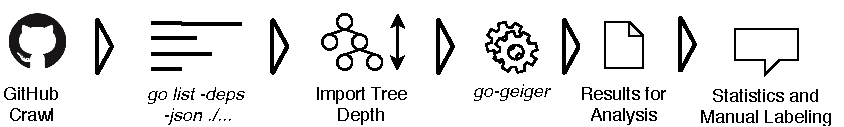
\includegraphics[width=\textwidth]{assets/figures/chapter1/outline.pdf}
    \caption{Thesis Outline and Chapter Relations}
    \label{fig:outline}
\end{figure}

